\chapter{The Execution Stack}

In this chapter we try to map the source code of GHC to high level text.
While there are academic literature on how GHC works, a lot of details have
since changed and the papers are now partially obsolete. Since even
small details of the execution stack will be important for implementating stack traces,
most information is based on the only definitive source of how the
stack is working: The GHC source code.

The sections in this chapter will stick to objective facts,
they'll not discuss difficulties of implementing stack traces.
Discussions will be kept for the next chapter.

\section{Number of stacks}

Haskell's \texttt{base} library exports the following primitive \cite{base_forkIO}:
\mint{haskell}|forkIO :: IO() -> IO()|
Intuitively \texttt{forkIO} just creates another "green" thread running its argument.
Since there will be two concurrent threads running after this, clearly
another execution stack have been created somehow. In this section we
look at how many execution stacks there will be by looking at
where they are referenced from.

The implementation of \texttt{forkIO} is
that it will create another \emph{Thread State Object} (TSO). As
can be seen from figure \ref{fig:tso_definition}, a TSO points at a
Stack object fully reproduced in figure \ref{fig:stack_definition}.
Thread State Objects themselves are usually referenced from \emph{Capabilities}.
A Capability contains all essential values for \emph{executing}
Haskell code. It can be thought as a virtual CPU, it contains
the virtual register values of the STG abstract machine. It contains
a singly-linked deque of all TSOs that are scheduled to run, meaning
there is a one to many relationship between a capability and a execution
stack. Capabilities themselves also come in multitude in the run time
system (with the default set of compilation symbols). The number of
capabilities is configurable through a runtime option, as a rule of
thumb it should be set to as many as the number of cores on the computer
\cite{commentary_capabilities}. In conclusion, the number of stacks is
the same as the total number of green threads (TSOs) as illustrated in
figure \ref{fig:stacks}.

\begin{figure}
\begin{mdframed}
  \begin{minted}{c}
typedef struct StgTSO_ {
    StgHeader               header;
    // deleted lines ...
    struct StgStack_       *stackobj;
    // ...
    struct Capability_*     cap;
    // ...
    StgWord32  tot_stack_size;
} *StgTSOPtr;
  \end{minted}
  \caption{The definition of \texttt{StgTSO} from the GHC run-time system
code}
  \label{fig:tso_definition}
\end{mdframed}
\end{figure}

\begin{figure}
\begin{mdframed}
  \begin{minted}{c}
typedef struct StgStack_ {
    StgHeader  header;
    StgWord32  stack_size;     // stack size in *words*
    StgWord32  dirty;          // non-zero => dirty
    StgPtr     sp;             // current stack pointer
    StgWord    stack[FLEXIBLE_ARRAY];
} StgStack;
  \end{minted}
  \caption{The definition of \texttt{StgStack} from the GHC run-time system
code}
  \label{fig:stack_definition}
\end{mdframed}
\end{figure}

\begin{figure}
  \centering
  \includegraphics[width=3.0in]{build/fig/stacks}
  \caption{Two virtual CPUs (Capabilities) running a total of three
green threads. Each green thread have it's own execution stack.
This is at a particular moment of the lifetime of a Haskell program,
the number of threads is dynamic.} % Fonot: TODO numera är capabilities också dynamiska
  \label{fig:stacks}
\end{figure}

\section{What's on the Stack?}

In STG-land, all heap object confirm to the template shown in figure \ref{fig:heap_object} \cite{commentary_heap_objects}.
A \emph{stack frame} is a heap object whose
associated info table is of any of the types listed in figure \ref{fig:stack_types}.

\begin{figure}
  \centering
  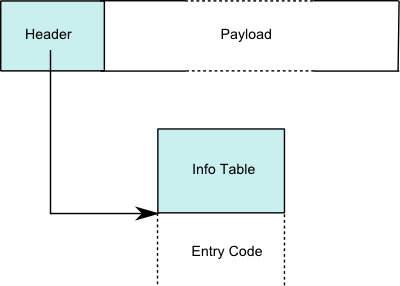
\includegraphics[width=3.0in]{fig/heap-object}
  \caption{Structure of heap objects in Haskell. TODO: Bilden är snodd!}
  \label{fig:heap_object}
\end{figure}

\begin{figure}
\begin{mdframed}
  \begin{minted}{c}
#define RET_BCO                 31
#define RET_SMALL               32
#define RET_BIG                 33
#define RET_FUN                 34
#define UPDATE_FRAME            35
#define CATCH_FRAME             36
#define UNDERFLOW_FRAME         37
#define STOP_FRAME              38
// ... some omitted non-stack closure types ...
#define ATOMICALLY_FRAME        57
#define CATCH_RETRY_FRAME       58
#define CATCH_STM_FRAME         59
  \end{minted}
  \caption{The subset of closure types that are present on the stack.
The excerpt is from \cite{github_closure_types}. Which types that exist
on the stack is based on \cite{github_scavenge_stack}.}
  \label{fig:stack_types}
\end{mdframed}
\end{figure}


In this section we'll dive into
some details about the stack frames. Other details
are omitted, like how garbage collection is treating the closures.

\subsection{Size of the closures}

% Behövs någonting här? Är det relevant?

% EXTERN_INLINE StgWord stack_frame_sizeW( StgClosure *frame );
% EXTERN_INLINE StgWord stack_frame_sizeW( StgClosure *frame )
% {
%     StgRetInfoTable *info;

%     info = get_ret_itbl(frame);
%     switch (info->i.type) {

%     case RET_FUN:
%       return sizeofW(StgRetFun) + ((StgRetFun *)frame)->size;

%     case RET_BIG:
%       return 1 + GET_LARGE_BITMAP(&info->i)->size;

%     case RET_BCO:
%       return 2 + BCO_BITMAP_SIZE((StgBCO *)((P_)frame)[1]);

%     default:
%       return 1 + BITMAP_SIZE(info->i.layout.bitmap);
%     }
% }

\subsection{Code of Stack Frames and its Arity}

We are used to think of the \emph{arity} of a function as number
of \emph{arguments} that it takes. That is valid in the context of the
STG-machine. But it doesn't necessarily match the way a Haskell
programmer thinks. By arity we mean how many arguments the compiled
STG function takes. See figure \ref{fig:tricky_arity}. \cite{commentary_function_calls}

\begin{figure}
\begin{mdframed}
        \begin{subfigure}[t]{0.5\textwidth}
          \begin{minted}{haskell}
f :: Bool -> Bool -> Bool
f = \x -> if x then not else id
          \end{minted}
          \caption{Haskell function}
        \end{subfigure}
    ~ %add desired spacing between images, e. g. ~, \quad, \qquad etc.
    %(or a blank line to force the subfigure onto a new line)
        \begin{subfigure}[t]{0.5\textwidth}
          \begin{minted}{haskell}
f = FUN(x -> case x of {
               True  -> not;
               False -> id });
          \end{minted}
          \caption{STG function, note that the number of arguments is
explicitly just one}
        \end{subfigure}
  \caption{In Haskell-land, the function can be fed up to two arguments.
  But we say that the arity is one, because the STG function that will be
  compiled takes one argument and returns a \texttt{FUN}. Note that \texttt{not}
  and \texttt{id} are themselves \texttt{FUN}s.
 }
  \label{fig:tricky_arity}
\end{mdframed}
\end{figure}

According to the return convention \cite{commentary_return_convention},
all stack frames info tables contain executable code that should be
instantly jumped to once a result is being returned. When the code
have arguments, they are pushed on the stack before jumping to the code.
In addition to arguments, there are \emph{fields} too.
Fields are similar to arguments but are already placed on the stack
and is part of the stack frame. When a function is entered,
the stack could look like in figure \ref{fig:stack_at_call}. Figure \ref{fig:field_and_arguments} shows examples
of Haskell code that will compile to code for info tables
of stack frames that have both fields and arguments.

\begin{figure}
\begin{mdframed}
  \includegraphics[width=3in]{build/fig/stack_at_call}
  \caption{The stack when the topmost function on the stack is invoked \cite{github_stack_at_call}.
In this case we pass the first argument by register, so \texttt{arg 1}
is stored in the (virtual) register \texttt{R1} described in the STG.}
  \label{fig:stack_at_call}
\end{mdframed}
\end{figure}

\begin{figure}
\begin{mdframed}
        \begin{subfigure}[t]{0.5\textwidth}
          \begin{minted}{haskell}
... = \x y -> ... case x of
                   4 -> x + y
                   _ -> x - y
          \end{minted}
          \caption{The case continuation will have \texttt{y} as a field
and \texttt{x} as an argument}
        \end{subfigure}
    ~ %add desired spacing between images, e. g. ~, \quad, \qquad etc.
    %(or a blank line to force the subfigure onto a new line)
        \begin{subfigure}[t]{0.5\textwidth}
          \begin{minted}{haskell}
... = \x y -> ... case x of
                   4 -> x + 5
                   _ -> x + 10
          \end{minted}
          \caption{The case continuation doesn't depend on \texttt{y},
so it will have no fields and \texttt{x} as it's only argument.}
        \end{subfigure}
  \caption{Two examples of code that will be turned into case
continuations.}
  \label{fig:field_and_arguments}
\end{mdframed}
\end{figure}

It should be noted that almost all return functions in the run time library
either take no arguments or only one argument. The notable exception is the
family of call continuations, discussed in subsection \ref{sec:call_continuation_frames}.

\section{The members of the stack}

In the previous section we defined what a stack frame is and enumerated
them, in this section we look categorize them further.

\subsection{Case continuation frames}

Case continuations is what comes naturally from having lazy evaluation
with pattern matching. When evaluating a case-expression, the code first
pushes the case continuation frame \emph{(\texttt{case} * \texttt{of}
\dots)} and then jumps to the entry code of the scrutiny.

\subsection{Update frames}

Consider the following code:

\begin{minted}[gobble=2]{haskell}
  let x = 2 + 3
  in x + x
\end{minted}

Here, \texttt{x} will only be evaluated once. This is implemented
through update frames. Update frames \emph{(Upd * \texttt{t})}
are pushed when a \texttt{THUNK \emph{x}} is evaluated, the frame's only
field will be the thunk itself \cite{github_thunk_code}. After the frame is
pushed the entry code for \texttt{x} is entered. When the code returns,
the result is passed to the update frame as an argument, which will
overwrite the thunk with an indirection to its argument (the result of
\texttt{x}) \cite{github_updates_indirection}.


\subsection{Call continuation frames} \label{sec:call_continuation_frames}

When evaluating \mint{haskell}|f True False|
where \texttt{f} is from figure \ref{fig:tricky_arity}, we have the
following scenario:

\begin{itemize}
  \item
    The function \texttt{f} has arity 1.
  \item
    We have an application of 2 arguments.
  \item
    The code has since long type checked. We assume there is no
programming error and that \texttt{f True} will return another function.
\end{itemize}

We can't just jump to the code of \texttt{f} and forget about the last
argument \texttt{False}. Instead, we first put a call continuation
frame \emph{(*\texttt{False})} and then jump to the code of \texttt{f}
\cite{evalapplyjfp06}. % TODO * --> ball
What would happen is that when \texttt{f True} evaluates and jumps to
the entry code of the call continuation, the call continuation would
first put its fields (\texttt{False}) on the stack (or write to
register \texttt{R1}) and then jump to the entry code of the argument it
got passed (the result of \texttt{f True}).
All call continuations are of closure type \texttt{RET\_SMALL}
\cite{github_genapply_RET_SMALL}.

\subsection{Overflow frames}

Overflow frames allow the stack itself to have dynamically growing or
shrinking size. Their significance is discussed in section \ref{sec:structure_of_stack}.

\subsection{Other frames}

Figure \ref{fig:stack_types} showed that there are other closure types
that play a role on the Haskell execution stack, including retry frames
for Software Transactional Memory. We will not examine these other
frames further.

\section{Structure of Stack} \label{sec:structure_of_stack}

It's a linked list! 

\section{Reifying the Stack}

At any given time, the stack can be reified. This is how: blah blah
